\documentclass[a4paper,10pt]{article}

\usepackage{graphicx}
\usepackage[ansinew]{inputenc}
\usepackage[spanish]{babel}
\usepackage{enumerate}
\usepackage{pdfpages}
\usepackage{listings}
\usepackage{color}

\lstset{
  language=C,                	  % choose the language of the code
  numbers=left,                   % where to put the line-numbers
  stepnumber=1,                   % the step between two line-numbers.
  numbersep=5pt,                  % how far the line-numbers are from the code
  backgroundcolor=\color{white},  % choose the background color. You must add \usepackage{color}
  showspaces=false,               % show spaces adding particular underscores
  showstringspaces=false,         % underline spaces within strings
  showtabs=false,                 % show tabs within strings adding particular underscores
  tabsize=2,                      % sets default tabsize to 2 spaces
  captionpos=b,                   % sets the caption-position to bottom
  breaklines=true,                % sets automatic line breaking
  breakatwhitespace=true,         % sets if automatic breaks should only happen at whitespace
  breakautoindent=false,
  breakindent=0pt
  %title=\lstname,                 % show the filename of files included with \lstinputlisting;
}

\title{	\textbf{Trabajo Pr\'actico \#0: Infraestructura B\'asica}}
\author{
	Fern\'andez Cynthia, \textit{Padr\'on Nro. 91.487}               \\
	\texttt{ cm.fernandez.28@gmail.com }                             \\[2.5ex]
	Quispe Gaston, \textit{Padr\'on Nro. 86.398}                     \\
	\texttt{ gaston.quispe@gmail.com }                               \\[2.5ex]
	Nombre y Apellido de Autor, \textit{Padr\'on Nro. 90.596}        \\
	\texttt{ valeria.mrb@gmail.com }                                 \\[2.5ex]
	\normalsize{1er. Cuatrimestre de 2017}                           \\
	\normalsize{66.20 Organizaci\'on de Computadoras  $-$ Pr\'actica Mi\'ercoles} \\
	\normalsize{Facultad de Ingenier\'ia, Universidad de Buenos Aires}            \\
       }
\date{}

\makeindex

\begin{document}

\maketitle


\thispagestyle{empty}   % quita el n�mero en la primer p�gina


\begin{abstract}
El objetivo de este trabajo pr\'actico es la adquisici\'on de
pr\'actica en la utilizaci\'on de herramientas de software, necesarias
para el curso de la materia, a trav\'es de la implementaci\'on de un
programa simple en lenguaje C para la detecci\'on de pal\'indromos.
Finalmente se obtendr\'a el c\'odigo MIPS32 de dicho programa.
\end{abstract}

\tableofcontents

\section{Documentaci\'on relevante}

Se decidi\'o implementar el c\'odigo C dentro de un main(). No
implementaremos clases ni librer\'ias propias porque la complejidad
l\'ogica del programa no lo amerita.\\
Para el control de la versi\'on utilizamos GitHub. Se trabajo con una
rama 'dev' local para realizar cambios y una rama 'master' local
para hacer push contra el 'master remoto'.\\

\subsection{Algunos detalles de implementaci\'on}

Con respecto a la implementaci\'on de la l\'ogica de detecci\'on de palabras
pal\'indromas, provista por la funci\'on int es\_capicua(char* palabra),
se utiliza la funci\'on char tolower(char caracter), provista por la
librer\'ia ctype, para cumplir con la condici\'on de ser case insensitive.\\
\\
Las formas posibles de interactuar con el programa son:
\begin{itemize}
	\item \textbf{./a.out -i $<$nombreArchivoEntrada$>$ -o $<$nombreArchivoSalida$>$}:
	Leer el contenido de archivo de entrada y lo escribe en el de salida
	\item \textbf{./a.out -i $<$nombreArchivoEntrada$>$}:
	Escribir en salida stdout, (por default la consola).
	\item \textbf{./a.out -o $<$nombreArchivoSalida$>$}:
	Lee entrada stdin. Dos opciones.
	\begin{itemize}
		\item Entrada interacitiva: La finalizaci\'on del ingreso
		de una linea se identifica al presionar enter. La
		finalizaci\'on de la ejecuci\'on de la escritura del
		archivo se identifica con ctr+d.
		\item Redirecci\'on mediante pipe: El archivo de entrada se
		recibe a traves de un comando previo.\\
		Ex: echo "soy un archivo sin palindromos" $|$ -o $<$nombreArchivoSalida$>$
	\end{itemize}
	\item \textbf{./a.output}: Lee entrada stdin y stdout.
\end{itemize}

Los nombres de archivos de \textbf{entrada} y \textbf{salida} pueden reemplazarse con con el
caracter \textbf{-}. Lo cual indica que dichos archivos son \textbf{stdin}
y \textbf{stdout} respectivamente.

\subsection{Asunciones}

De la interpretaci\'on del enunciado y las dudas resueltas en grupo, cabe destacar lo siguiente:\\
\begin{itemize}
	\item Consideramos pal\'indromos palabras de \textbf{un solo caracter v\'alido}.
	\item Dado que los espacios no son caracteres incluidos, entendemos
	que se s\'olo se evaluar\'an palabras pal\'indromas y no frases.
	Ergo, el programa no est\'a dise\~nado para detectar
	frases pal\'indromas.
	\item El programa no est\'a dise\~nado para detectar repeticiones,
	es decir, si se ingresa dos veces la misma palabra a la entrada y
	\'esta cumple la condici\'on de ser pal\'indroma, se devolver\'a
	\textbf{dos veces} esa palabra a la salida.
	\item Utilizamos los caracteres inv\'alidos, es decir, aquellos que
	no est\'an contemplados en los componentes l\'exicos del stream de
	entrada, \textbf{como separadores}. De modo que si una palabra incluye un
	car\'acter inv\'alida quedar\'a separada en dos palabras
	autom\'aticamente.
	Por ejemplo, si ingresamos AA@BB, el sistema tomar\'a como que
	se ingresaron las palabras AA y BB.
	\item Cuando existe un error de lectura o escritura, se contin\'ua
	con la ejecuci\'on y se muestra un mensaje de error por
	\textbf{stderr}. Siendo necesario abortar dicha ejecuci\'on
	con el comando ctrl + d.
\end{itemize}


\section{Comandos para compilar}

Para compilar el programa utilizamos GCC (GNU Compiler Collection) incluido
en el sistema operativo NetBSD. Dicho sistema es emulado mediante el programa
\textbf{gxemul} y accedido mediante un tunel ssh reverso desde un sistema
linux (en nuestro caso, \textbf{Ubuntu 16.04}).\\

\begin{enumerate}[1.]
	\item Movemos los archivos del proyecto a compilar desde linux al
	home en NetBSD:\\
	\textbf{scp -P2222 -r /home/tporga root@127.0.0.1: }$\sim$

	\item El comando que corremos en la terminal de NetBSD para compilar
	el c\'odigo fuente en lenguaje C es:\\
	\textbf{gcc main.c -Wall}\\
	Si no indicamos par\'ametros de salida, se genera un archivo ejecutable
	llamado \textbf{a.out}, dentro del directorio donde se encuentra el
	c\'odigo fuente. Para ejecutarlo utilizamos el comando \textbf{./a.out}.

	\item Para obtener el c\'odigo en ensamblador generado por gcc
	corremos la siguiente linea en el shell.\\
	\textbf{gcc -Wall -O0 -S -mrnames main.c}\\
	Donde:
	\begin{itemize}
		\item Wall: Activa todos los mensajes de warning del compilador.
		\item S: Detiene al compilador luego de generar el assembly.
		\item mrnames (solo para MIPS): Indica al compilador que
		genere la salida utilizando nombre de registro en lugar
		de n\'umero de registro.
		\item O0: No aplica optimizaciones.
	\end{itemize}
	Este comando genera un archivo llamado \textbf{main.s} que contiene el
	c\'odigo ensamblador que gcc genera para \textbf{main.c}.
	\item Para traer los documentos compilados de nuevo a linux:\\
	\textbf{scp -P2222 -r root@127.0.0.1:/home/tporga }$\sim$
\end{enumerate}
\newpage
\section{Corridas de pruebas}
Se realizan ejecutando el script de pruebas automatizadas \textbf{tests.sh} con
el comando:\\
\textbf{.\textbackslash tests.sh}.\\
Este script espera que:
\begin{itemize}
	\item Los archivos de entrada y salida esperadas de encuentren
	en la carpeta \textbf{Tests}.
	\item El archivo ejecutable se llame \textbf{a.out} y se ecuentre en la misma
	carpeta que \textbf{tests.sh}.
\end{itemize}


Las pruebas leen el ejecutable a.out. Se corre el archivo tests.sh para ejecutar todas las pruebas, con el comando bash test.sh.\\
\\
Las 10 pruebas realizadas son:\\
\begin{enumerate}[1.]
	\item PRUEBA: Entrada vac\'ia.\\
	RESULTADO: Salida vac\'ia.\\

	\item PRUEBA: Entrada de dos frases, con caracteres v\'alidos, tres pal\'indromos.\\
	\begin{itemize}
		\item ENTRADA:
		\lstinputlisting{../Tests/Entrada2.txt}
		\item RESULTADO:
		\lstinputlisting{../Tests/SalidaEsperada2.txt}
	\end{itemize}

	\item PRUEBA: Entrada de tres l\'ineas, con caracteres v\'alidos, incluyendo gui\'on medio.\\
	\begin{itemize}
		\item ENTRADA:
		\lstinputlisting{../Tests/Entrada3.txt}
		\item RESULTADO:
		\lstinputlisting{../Tests/SalidaEsperada3.txt}
	\end{itemize}

	\item PRUEBA: Entrada de mil caracteres con un \'unico pal\'indromo.\\
	\begin{itemize}
		\item ENTRADA:
		\lstinputlisting{../Tests/Entrada4.txt}
		\item RESULTADO:
		\lstinputlisting{../Tests/SalidaEsperada4.txt}
	\end{itemize}

	\item PRUEBA: Entrada de varios pal\'indromos con caracteres inv\'alidos.\\
	\begin{itemize}
		\item ENTRADA:
		\lstinputlisting{../Tests/Entrada5.txt}
		\item RESULTADO:
		\lstinputlisting{../Tests/SalidaEsperada5.txt}
	\end{itemize}

	\item PRUEBA: Entrada de una palabra pal\'indroma dentro de caracteres inv\'alidos.\\
	\begin{itemize}
		\item ENTRADA:
		\lstinputlisting{../Tests/Entrada6.txt}
		\item RESULTADO:
		\lstinputlisting{../Tests/SalidaEsperada6.txt}
	\end{itemize}

	\item PRUEBA:Entrada de pal\'indromos con guiones y n\'umeros.\\
	\begin{itemize}
		\item ENTRADA:
		\lstinputlisting{../Tests/Entrada7.txt}
		\item RESULTADO:
		\lstinputlisting{../Tests/SalidaEsperada7.txt}
	\end{itemize}

	\item PRUEBA: Entrada de varios pal\'indromos entre caracteres inv\'alidos en una sola l\'inea.\\
	\begin{itemize}
		\item ENTRADA:
		\lstinputlisting{../Tests/Entrada8.txt}
		\item RESULTADO:
		\lstinputlisting{../Tests/SalidaEsperada8.txt}
	\end{itemize}

	\item PRUEBA: Entrada de palabras no palindromas entre caracteres inv\'alidos.\\
	\begin{itemize}
		\item ENTRADA:
		\lstinputlisting{../Tests/Entrada9.txt}
		\item RESULTADO: Vac\'ia.
	\end{itemize}

	\item PRUEBA: Entrada de caracteres inv\'alidos.\\
	\begin{itemize}
		\item ENTRADA:
		\lstinputlisting{../Tests/Entrada10.txt}
		\item RESULTADO: Vac\'ia.
	\end{itemize}
\end{enumerate}

\section{Problemas e inconvenientes que se presentaron durante el desarrollo del trabajo pr\'actico}
Los principales inconvenientes surgieron de la inexperiencia en la utilizaci\'on de las herramientas propuestas para el desarrollo del trabajo pr\'actico. Las enumeramos a continuaci\'on:

\begin{itemize}
	\item Necesidad de instalar Open SSH para generar el t\'unel.
	\item Necesidad de borrar el archivo know\_host para establecer
	conexi\'on a la ip.
	\item Decidimos no utilizar un IDE ya que la extensi\'on del
	c\'odigo no iba a superar las 200 l\'ineas.
	Simplemente utilizamos un editor de texto.
	En la experiencia nos hubiese resultado \'util tener
	un herramienta para debuguear.
	\item Los test observados en la secci\'on 5.1 del enunciado no
	se adaptan a la definici\'on pal\'indromo que encontramos y,
	adem\'as, es ambigua. Por lo tanto, y en base a respuestas del
	grupo yahoo, establecimos que el ejemplo del test donde
	el 0 no es palindromo \textbf{es incorrecto}.\\
	Los inconvenientes que surgieron a partir de la interpretaci\'on
	del enunciado fueron resueltas en la subsecci\'on '\textbf{Asunciones}'.
\end{itemize}
f
\newpage
\section{C\'odigo Fuente C}
\lstinputlisting{../main.c}

\newpage
\section{C\'odigo MIPS32}
\lstinputlisting{../main.s}

\newpage
\section{C\'odigo de pruebas automatizadas}
\lstinputlisting{../tests.sh}

\newpage
\section{Enunciado}

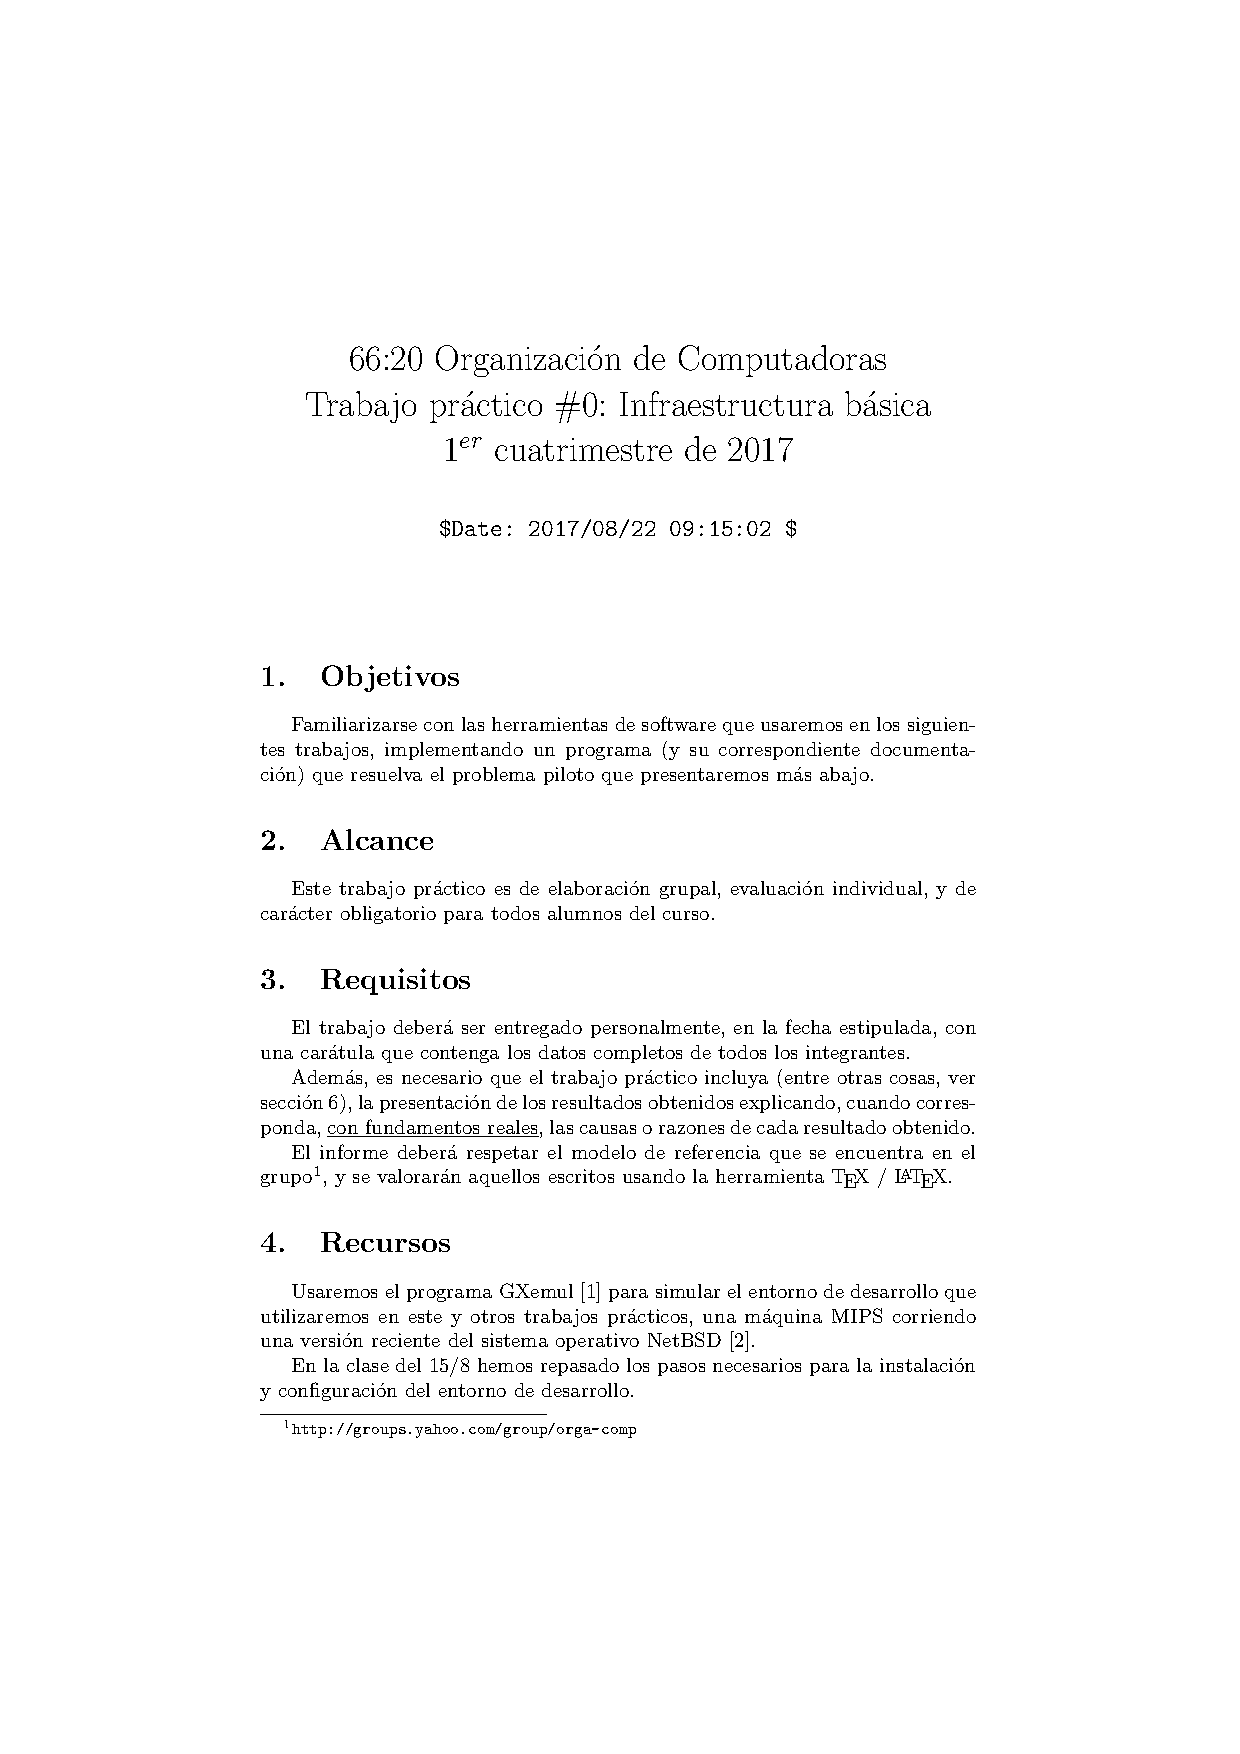
\includepdf[pages=-]{tp0-enunciado.pdf}

\end{document}
